\documentclass[conference]{IEEEtran}
\IEEEoverridecommandlockouts
\usepackage{cite}
\usepackage{amsmath,amssymb,amsfonts}
\usepackage{graphicx}
\usepackage{textcomp}
\usepackage{booktabs}
\usepackage{stfloats}
\usepackage{placeins}
\usepackage[hyphens]{url}
\def\UrlBreaks{\do\/\do-}
\renewcommand{\arraystretch}{0.92}
\setcounter{dbltopnumber}{2}
\renewcommand{\dbltopfraction}{0.85}

\begin{document}
\raggedbottom

\title{Beyond the Calibration Range: Mechanisms of Variable-Selection Robustness in Raman Quantification of Olive Oil Adulteration}

\author{
\IEEEauthorblockN{Abdelrahman A. Alshames, Omnia S. Eshra, Zeina Eltannikhy,\\ Moaz H. El Garawany, and Alaa A. Sanhoury}
\IEEEauthorblockA{{Faculty of Computer Science and Information Technology, Egypt-Japan University of Science and Technology (E-JUST)}\\
{New Borg El-Arab City, Alexandria 21934, Egypt}\\
{\footnotesize abdelrahman.aboegela@ejust.edu.eg, omnia.eshra@ejust.edu.eg}\\
{\footnotesize zeina.eltannikhy@ejust.edu.eg, moaz.320240032@ejust.edu.eg}\\
{\footnotesize alaa.320250111@ejust.edu.eg}}
}

\maketitle

% Generated from the complete standardized 15-seed matrix.
\newcommand{\UnitPLSR}{4.42}
\newcommand{\UnitPLSRSD}{0.00}
\newcommand{\UnitPLSRTime}{0.1}
\newcommand{\RegionUnitPLSR}{3.82}
\newcommand{\UnitVIP}{1.67}
\newcommand{\UnitVIPSD}{0.36}
\newcommand{\UnitVIPTime}{8.8}
\newcommand{\RegionUnitVIP}{1.48}
\newcommand{\UnitIPLS}{2.43}
\newcommand{\UnitIPLSSD}{0.74}
\newcommand{\UnitIPLSTime}{1.2}
\newcommand{\RegionUnitIPLS}{2.22}
\newcommand{\UnitGA}{1.87}
\newcommand{\UnitGASD}{0.55}
\newcommand{\UnitGATime}{458.0}
\newcommand{\RegionUnitGA}{2.18}
\newcommand{\UnitGWO}{2.30}
\newcommand{\UnitGWOSD}{0.84}
\newcommand{\UnitGWOTime}{77.4}
\newcommand{\RegionUnitGWO}{1.78}
\newcommand{\UnitGARed}{2.79}
\newcommand{\UnitGARedSD}{1.54}
\newcommand{\UnitGWORed}{2.62}
\newcommand{\UnitGWORedSD}{1.04}
\newcommand{\UnitCapTwenty}{3.87}
\newcommand{\UnitCapTwentySD}{0.50}
\newcommand{\UnitCapTwentyLV}{10--19}
\newcommand{\UnitVIPK}{130--300}
\newcommand{\UnitGAFixedTen}{1.92}
\newcommand{\UnitFullFixedTen}{4.42}
\newcommand{\UnitVarianceHalf}{2.28}
\newcommand{\UnitVarianceHalfFixedTen}{1.98}
\newcommand{\UnitGADelta}{-2.47}
\newcommand{\UnitGACI}{[-3.61,-1.33]}
\newcommand{\UnitGWODelta}{-1.96}
\newcommand{\UnitGWOCI}{[-3.09,-0.99]}
\newcommand{\UnitRandom}{3.99}
\newcommand{\UnitRandomSD}{1.53}
\newcommand{\UnitResidualR}{0.93}
\newcommand{\MeanPLSR}{3.09}
\newcommand{\MeanPLSRSD}{0.80}
\newcommand{\MeanPLSRTime}{0.1}
\newcommand{\RegionMeanPLSR}{2.00}
\newcommand{\MeanVIP}{3.10}
\newcommand{\MeanVIPSD}{0.64}
\newcommand{\MeanVIPTime}{9.1}
\newcommand{\RegionMeanVIP}{1.88}
\newcommand{\MeanIPLS}{2.91}
\newcommand{\MeanIPLSSD}{1.48}
\newcommand{\MeanIPLSTime}{1.7}
\newcommand{\RegionMeanIPLS}{2.64}
\newcommand{\MeanGA}{3.36}
\newcommand{\MeanGASD}{0.73}
\newcommand{\MeanGATime}{392.2}
\newcommand{\RegionMeanGA}{2.81}
\newcommand{\MeanGWO}{3.67}
\newcommand{\MeanGWOSD}{1.05}
\newcommand{\MeanGWOTime}{71.2}
\newcommand{\RegionMeanGWO}{2.93}
\newcommand{\MeanGARed}{3.66}
\newcommand{\MeanGARedSD}{1.19}
\newcommand{\MeanGWORed}{3.66}
\newcommand{\MeanGWORedSD}{1.45}
\newcommand{\MeanCapTwenty}{3.09}
\newcommand{\MeanCapTwentySD}{0.80}
\newcommand{\MeanCapTwentyLV}{4--9}
\newcommand{\MeanVIPK}{250--600}
\newcommand{\MeanGAFixedTen}{2.17}
\newcommand{\MeanFullFixedTen}{1.72}
\newcommand{\MeanVarianceHalf}{3.20}
\newcommand{\MeanVarianceHalfFixedTen}{1.92}
\newcommand{\MeanGADelta}{+0.25}
\newcommand{\MeanGACI}{[-0.64,+1.10]}
\newcommand{\MeanGWODelta}{+0.62}
\newcommand{\MeanGWOCI}{[-0.24,+1.58]}
\newcommand{\MeanRandom}{3.59}
\newcommand{\MeanRandomSD}{1.43}
\newcommand{\MeanResidualR}{0.99}
\newcommand{\GAInteraction}{+2.71}
\newcommand{\GAInteractionCI}{[+1.39,+4.25]}
\newcommand{\GWOInteraction}{+2.59}
\newcommand{\GWOInteractionCI}{[+1.22,+4.20]}


\begin{abstract}
Raman models for quantifying extra virgin olive oil (EVOO) in vegetable blends are commonly evaluated within their calibration range, although screening samples can exceed it. We investigate what makes variable selection robust under this shift using 605 public EVOO--sunflower spectra: calibration covers 0--31\% EVOO and the main test comprises 140 spectra at 50--100\%. Full-spectrum partial least squares regression (PLSR), genetic-algorithm and grey-wolf moving-window selection, Variable Importance in Projection (VIP), and interval PLS are compared under unit-variance scaling and mean centering. Every fitted condition uses 15 matched, mixture-grouped CV assignments; optimizer randomness uses the corresponding seed IDs. At published search budgets, unit-variance PLSR, GA-MW and GWO-MW give mean prediction errors of \UnitPLSR, \UnitGA\ and \UnitGWO\ EVOO percentage points; under mean centering the corresponding errors are \MeanPLSR, \MeanGA\ and \MeanGWO. Refitting identical selected channels at matched latent-variable counts separates scaling from model complexity. A simple calibration-variance filter obtains unit-variance error \UnitVarianceHalf, supporting a weighting explanation for part of the selection benefit. VIP reaches \UnitVIP\ under unit variance. Five calibration windows show that the preferred selection strategy depends on both scaling and concentration coverage. These results identify conditions for robustness rather than a uniformly superior selector.
\end{abstract}

\begin{IEEEkeywords}
Raman spectroscopy, chemometrics, variable selection, calibration-range shift, olive oil authentication
\end{IEEEkeywords}

\section{Introduction}
Raman spectroscopy offers rapid screening of vegetable blends whose declared extra virgin olive oil (EVOO) fraction may be inaccurate. Zhu \textit{et al.}~\cite{zhu2023} combined partial least squares regression (PLSR) with metaheuristic moving-window selection, obtaining improved quantification within six EVOO levels spanning 5--30\%. Such a calibration can be useful for screening, but a sample with a higher true EVOO fraction requires extrapolation. An advantage measured within the calibrated interval need not persist beyond it.

This distinction is established in multivariate calibration. Estienne \textit{et al.}~\cite{estienne2001} examined both predictor-space and concentration extrapolation, including the influence of irrelevant variables; Huo \textit{et al.}~\cite{huo2024} compared linear and nonlinear models across concentration ranges. These studies motivate testing beyond calibration rather than treating in-range accuracy as a sufficient indicator of deployment performance. Here we hold the PLS backbone fixed and ask which modeling choices account for the apparent extrapolation benefit of spectral selection.

Selection is coupled to preprocessing. Scaling each channel to unit variance gives low- and high-variance channels equal marginal weight, whereas mean centering preserves their relative variance. Wavelength selection and input weighting have accordingly been studied together~\cite{silalahi2020}. Raman calibration-transfer work also shows that preprocessing selected within a source domain need not transfer well~\cite{umprecht2025}. These findings motivate a controlled question under concentration extrapolation: does a selector's advantage reflect reproducibly useful spectral information, compensation for channel weighting, or a different model complexity?

We address that question using the public Picouet EVOO--sunflower dataset~\cite{picouet2023}, whose 0--100\% coverage permits a narrow calibration and genuinely disjoint higher-concentration levels. Our contributions are: (1) a controlled comparison of selection under two scaling conventions, including genetic-algorithm and grey-wolf searches at their published budgets; (2) interventions that hold the channels or latent-variable count fixed, supplemented by random and calibration-variance controls; and (3) a comparison with deterministic VIP and interval PLS across five calibration windows, identifying when inexpensive selection is sufficient and when it is unnecessary. Together these experiments characterize the channel-weighting and model-complexity effects underlying robustness in this quantification task.

\section{Materials and Methods}
\subsection{Spectra, Calibration Windows and Held-Out Tests}
The Picouet dataset contains 605 Raman spectra of EVOO--sunflower mixtures (785\,nm excitation, approximately 500--2500\,cm$^{-1}$, 710 channels), provided as CALIBRATION (350), VALIDATION (165) and PREDICTION (90) rows~\cite{picouet2023}. The principal calibration uses the CALIBRATION rows at EVOO levels $\{0,10,15,23,25,31\}$\% ($n=135$). VALIDATION and PREDICTION supply the high-concentration test ($\geq50$\%, $n=140$); no concentration or mixture group in this test occurs in the narrow calibration. The low-concentration reference ($\leq35$\%) has 105 rows, of which 15 share a mixture group with calibration. We exclude those 15 when reporting RMSEP$_{\mathrm{low}}$, leaving 90 spectra. Ten spectra at 47--48\% form the guard band. Low-concentration error is a reference, not the primary extrapolation endpoint.

Four additional calibration windows contain the CALIBRATION levels in 0--15\% ($n=80$), 0--50\% ($n=200$), 63--100\% ($n=125$), and 23--54\% ($n=130$). For bounds $[l,h]$, the above and below tests contain held-out spectra at $y\ge h+19$ and $y\le l-19$, respectively. This preserves the principal experiment's 19-percentage-point separation. Every above/below test is concentration-disjoint from its calibration. The window extension compares PLSR, VIP and iPLS; optimizer budget effects are evaluated in the principal narrow regime. These windows test dependence within one dataset; they are not independent instruments or adulterants.

\subsection{Preprocessing and Grouped Model Development}
Each spectrum receives airPLS baseline correction~\cite{zhang2010} ($\lambda=10^5$, at most 15 iterations), standard normal variate (SNV) normalization, and Savitzky--Golay smoothing (11 channels, order 3). These fixed operations act independently on each spectrum. Column means and standard deviations are estimated only from the training rows of each fitted model. The two PLS conventions are mean centering alone and mean centering followed by unit-variance scaling~\cite{wold2001}. They are compared as experimental factors, not chosen by held-out error.

The weighting connection is explicit for the first PLS component. Let $X_c,y_c$ be centered calibration data, $M$ a diagonal channel-selection mask, and $D$ the diagonal matrix of training channel standard deviations (or $I$ for mean centering). For a single response,
\begin{equation}
\mathbf t_1\;\propto\;X_c M D^{-2} X_c^{\mathsf T}y_c.
\label{eq:weighting}
\end{equation}
Thus selection changes the same channel-weighted geometry as scaling. This identity motivates the controls; the behavior of the final multi-LV predictor is tested empirically rather than inferred from its first component alone.

Zhu \textit{et al.} explicitly used mean centering and modeled the 1000--1800\,cm$^{-1}$ region~\cite{zhu2023}. Our broader-spectrum experiment therefore adapts their moving-window design to the public data; it is not a reproduction of their original blend datasets. A matched-region check crops the raw spectra to 1000--1800\,cm$^{-1}$ before preprocessing and repeats both scaling conventions.

Acquisition date and EVOO fraction define mixture groups. They recover 109 groups: 98 contain five spectra and 11 combine two or more nominal mixtures. This conservative grouping keeps potentially related replicates together. Every fitted condition uses the same 15 master seed IDs (0--14). For each seed, shuffled \texttt{GroupKFold} produces matched group-preserving assignments across methods and scalings: three folds for search fitness and five for LV or VIP variable-count selection, including VIP's nested and final fits. The seed also initializes stochastic selection. Thus deterministic methods vary through CV assignment, while optimizers additionally vary through their search. All fitted parameters and model selection use calibration rows only; exact fold indices are archived for verification.

\subsection{Models and Explanatory Controls}
Full-spectrum PLSR uses 1--10 latent variables (LV), selected by five-fold grouped CV. GA-MW and GWO-MW~\cite{mirjalili2014} search 30 overlapping windows of five channels, yielding at most 150 distinct channels. Fitness is the mean three-fold CV RMSE of a five-LV PLSR; the final selected-channel model again chooses 1--10 LV. GA crossover and mutation probabilities are 0.6 and 0.03. The published budgets are population 100 (GA) or 20 (GWO), with 1000 iterations; reduced budgets use populations 40 and 20 with 40 iterations. Each optimizer is repeated at seeds 0--14 under each scaling and budget. A baseline-only sensitivity expands full-spectrum PLSR to 1--20 LV under both scalings with the same 15 assignments, checking whether the common 10-LV cap explains its performance.

VIP ranks channels from a full-spectrum 10-LV PLSR, selects the top $k$, and refits. The ranking is recomputed on each outer CV training fold; inner grouped CV selects the refit's LV count. The fixed 25-value $k$ grid spans 60--710 and includes the full spectrum, so selection is not forced when calibration CV favors retaining all channels. In the cropped-region check, counts are capped at the available channels and duplicates removed. Our forward interval-PLS baseline (iPLS), based on interval selection~\cite{norgaard2000}, partitions the spectrum into 20 contiguous intervals. It adds the interval giving the lowest five-fold grouped-CV error at 10 LV until no addition improves that error; the final PLSR selects 1--10 LV by grouped CV. Both methods use all 15 master assignments and are deterministic for a given assignment.

To separate channels from complexity, we refit all 15 GA-MW, GWO-MW and VIP selected sets per source scaling under \emph{both} refit scalings at each fixed LV count from 1 to 15; these are conditional interventions, not new independent searches. Random controls use one draw per master seed: 30 five-channel windows or a random set of 160 channels, followed by the same grouped LV selection as other methods. Simple variance filters retain the 160, 355, 533 or 639 highest-variance calibration channels; the ranking is recomputed inside each CV training fold and all 15 assignments are evaluated. Thresholds are reported as a sensitivity analysis, not optimized on test error. The full spectrum at a fixed LV count has no random or CV-dependent choice and is therefore a single common deterministic reference curve.

Repeatability is summarized per channel by pooled within-group variance divided by total calibration variance. This describes within-mixture variation relative to overall variation; it does not independently measure instrument noise or distinguish concentration effects from other between-group differences.

\begin{table*}[!t]
\caption{Narrow calibration: strict low-concentration error ($n=90$) and high-concentration error ($n=140$), in EVOO percentage points. Every row: mean $\pm$ population SD over the same 15 master-seed pipeline repetitions. Vars.: mean selected-channel count; LV: selected count or range. $\Delta$: difference in pooled RMSEP$_{\mathrm{high}}$ from PLSR at the same scaling, with multiplicity-adjusted bootstrap intervals for the published-budget comparisons.}
\label{tab:main}
\centering\footnotesize
\setlength{\tabcolsep}{4pt}
\begin{tabular}{@{}lllrrccc@{}}
\toprule
Scaling & Method & Budget & Vars. & LV & RMSEP$_{\mathrm{low}}$ & RMSEP$_{\mathrm{high}}$ & $\Delta$ [interval]\\
\midrule
Unit var. & PLSR & --- & 710 & 10 & 0.98 $\pm$ 0.00 & 4.42 $\pm$ 0.00 & --- \\
Unit var. & VIP-PLSR & --- & 223 & 6--10 & 0.75 $\pm$ 0.04 & 1.67 $\pm$ 0.36 & --- \\
Unit var. & iPLS & --- & 217 & 10 & 0.86 $\pm$ 0.08 & 2.43 $\pm$ 0.74 & --- \\
Unit var. & GA-MW & Reduced & 131 & 5--9 & 0.85 $\pm$ 0.13 & 2.79 $\pm$ 1.54 & --- \\
Unit var. & GWO-MW & Reduced & 131 & 6--10 & 0.83 $\pm$ 0.14 & 2.62 $\pm$ 1.04 & --- \\
Unit var. & GA-MW & Published & 128 & 5--7 & 0.76 $\pm$ 0.05 & 1.87 $\pm$ 0.55 & $-2.47$ [$-3.61$, $-1.33$] \\
Unit var. & GWO-MW & Published & 108 & 5--10 & 0.79 $\pm$ 0.06 & 2.30 $\pm$ 0.84 & $-1.96$ [$-3.09$, $-0.99$] \\
\midrule
Mean-cent. & PLSR & --- & 710 & 4--9 & 0.69 $\pm$ 0.05 & 3.09 $\pm$ 0.80 & --- \\
Mean-cent. & VIP-PLSR & --- & 422 & 4--8 & 0.68 $\pm$ 0.04 & 3.10 $\pm$ 0.64 & --- \\
Mean-cent. & iPLS & --- & 371 & 5--10 & 0.75 $\pm$ 0.04 & 2.91 $\pm$ 1.48 & --- \\
Mean-cent. & GA-MW & Reduced & 138 & 4--7 & 0.78 $\pm$ 0.07 & 3.66 $\pm$ 1.19 & --- \\
Mean-cent. & GWO-MW & Reduced & 136 & 4--6 & 0.78 $\pm$ 0.07 & 3.66 $\pm$ 1.45 & --- \\
Mean-cent. & GA-MW & Published & 138 & 4--6 & 0.76 $\pm$ 0.05 & 3.36 $\pm$ 0.73 & $+0.25$ [$-0.64$, $+1.10$] \\
Mean-cent. & GWO-MW & Published & 121 & 4--7 & 0.77 $\pm$ 0.07 & 3.67 $\pm$ 1.05 & $+0.62$ [$-0.24$, $+1.58$]
\\
\bottomrule
\end{tabular}
\end{table*}

\subsection{Endpoints, Uncertainty and Execution}
RMSEP is the root mean squared prediction error in EVOO percentage points. Every fitted-method summary gives mean and population SD over the same 15 master-seed pipeline repetitions, including all windows, the cropped region, random and variance controls, and the full-range leakage reference. These repetitions describe fold-assignment and, where applicable, search variation on one dataset, not independent biological replications. A zero SD can occur when different CV assignments select the same final model.

Let $R_{m,s}$ denote pooled RMSEP over pipeline repetitions and high-concentration test spectra for method $m$ and scaling $s$. The primary contrasts are $\Delta_{m,s}=R_{m,s}-R_{\mathrm{PLSR},s}$ and $I_m=\Delta_{m,\mathrm{mean}}-\Delta_{m,\mathrm{unit}}$, for GA and GWO. Positive $I_m$ means selection is less beneficial under mean centering. Intervals use 10\,000 paired bootstrap resamples of the 28 test-mixture groups and master seed IDs, retaining the pairing across all methods and scalings. Bonferroni percentile intervals cover the six specified contrasts with nominal family-wise coverage of 95\%; they condition on the observed calibration data. Window and control comparisons are descriptive. Search fitness, measured after selection, is not presented as an unbiased estimate of generalization.

Grouped experiments ran on an Intel Core i5-10500H (6 cores, 12 threads), 15.8\,GB RAM, Windows build 26200, Python 3.11.5, NumPy 2.2.6, SciPy 1.16.1 and scikit-learn 1.7.2~\cite{pedregosa2011}. Parallel workers each use one linear-algebra thread. Calibration timings are measured separately on the idle machine with one thread and master seed 0: the median of three complete selection-and-fitting repetitions for \emph{every} method, including both published-budget optimizers and final LV selection. Shared preprocessing and data loading are excluded. Timing repeats measure execution variability; the 15-run protocol measures prediction variability.

\begin{figure*}[!t]
\centering
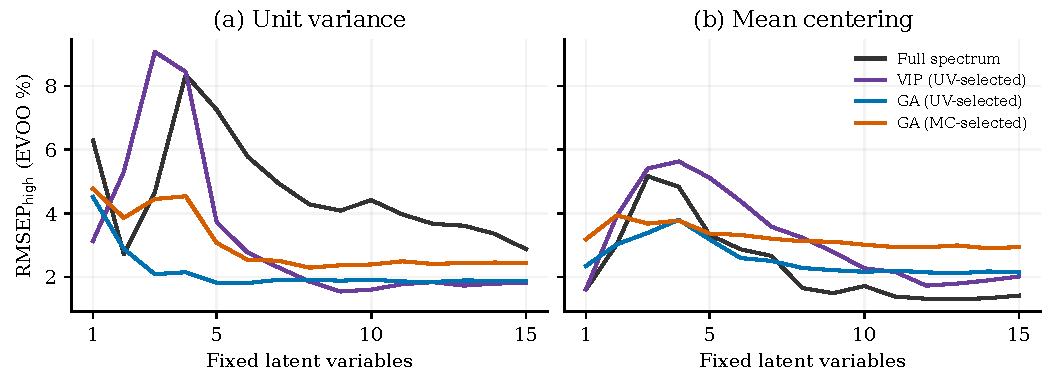
\includegraphics[width=0.90\linewidth]{figs/fig_final_fixed.pdf}
\caption{Conditional refits of fixed channel sets at 1--15 LV under (a) unit-variance scaling and (b) mean centering. GA and VIP curves average all 15 matched selections; the full-spectrum fixed-LV model is a common deterministic reference. UV/MC identify the scaling used to select the channels. Different behavior of the same channels under the two refit scalings separates weighting from channel identity; LV counts are displayed diagnostically and are not chosen using test errors.}
\label{fig:fixed}
\end{figure*}

\section{Results and Discussion}
\subsection{The Selection Advantage Depends on Scaling}
Table~\ref{tab:main} compares both scalings under identical calibration and test definitions. Full-spectrum PLSR gives RMSEP$_{\mathrm{high}}$ of \UnitPLSR\ under unit-variance scaling and \MeanPLSR\ under mean centering. At the published budget GA-MW gives \UnitGA\ and \MeanGA, while GWO-MW gives \UnitGWO\ and \MeanGWO. Thus a method comparison that fixes one scaling convention can give a materially different impression of the value of selection.

The scaling interactions are \GAInteraction\ for GA-MW (adjusted interval $\GAInteractionCI$) and \GWOInteraction\ for GWO-MW ($\GWOInteractionCI$). Both interaction intervals exclude zero. The within-scaling intervals in Table~\ref{tab:main} support improvement under unit variance, whereas the mean-centered intervals include zero. The evidence therefore establishes attenuation of the selection benefit, without establishing harm under mean centering or universal superiority of either scaling. The reduced-budget means are also shown: they establish how the conclusion depends on optimization effort instead of assuming that the reduced search is representative.

Expanding only the full-spectrum baseline's LV range to 20 gives unit-variance RMSEP $\UnitCapTwenty\pm\UnitCapTwentySD$ (selected LV: \UnitCapTwentyLV) and mean-centered RMSEP $\MeanCapTwenty\pm\MeanCapTwentySD$ across the same 15 assignments. Additional baseline capacity improves the unit-variance reference but does not remove the benefit of VIP selection. This sensitivity does not retune the other methods or replace the common-cap comparison.

The spectral region is another relevant condition. On 1000--1800\,cm$^{-1}$, grouped full-spectrum PLSR gives \RegionUnitPLSR\ under unit variance and \RegionMeanPLSR\ under mean centering; VIP gives \RegionUnitVIP\ and \RegionMeanVIP, and iPLS \RegionUnitIPLS\ and \RegionMeanIPLS. This check reinforces the need to distinguish an optimizer's contribution from the information and weighting supplied to it. Its reduced-budget search details are provided with the reproducibility outputs.

\begin{figure*}[!b]
\centering
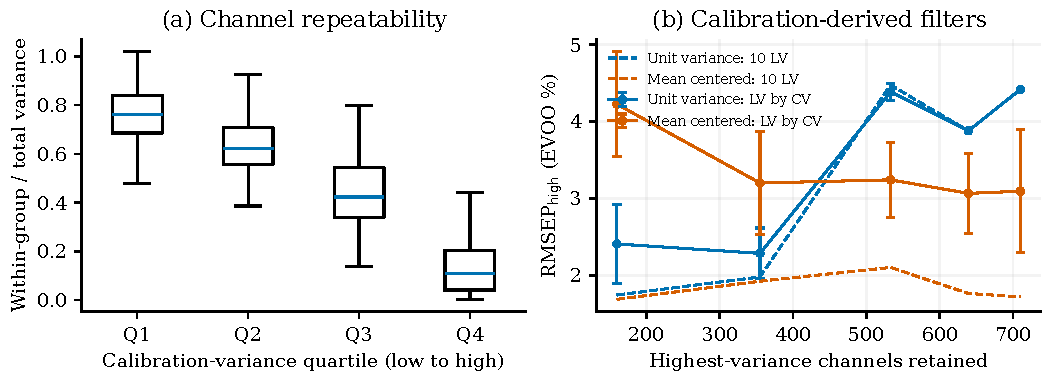
\includegraphics[width=0.90\linewidth]{figs/fig_final_variance.pdf}
\caption{(a) Within-group/total calibration variance by channel-variance quartile (boxplots; outliers suppressed). Lower values indicate more repeatable variation relative to total variation. (b) Retaining the highest-variance channels under both scalings: mean $\pm$ population SD across 15 matched grouped-CV assignments (solid) or the common 10-LV fit (dashed). The sensitivity curve separates the effects of retained channel count, scaling and LV selection.}
\label{fig:variance}
\end{figure*}

\subsection{Separating Channel Weighting from Model Complexity}
Fig.~\ref{fig:fixed} holds the selected channels fixed while varying scaling and LV count. The full spectrum's extrapolation error is strongly non-monotonic in LV, so reducing dimensionality alone does not guarantee accuracy. At 10 LV, unit-variance full-spectrum PLSR gives \UnitFullFixedTen, compared with \UnitGAFixedTen\ for the unit-variance-selected GA sets. Refitting those \emph{same} GA sets with mean centering gives \MeanGAFixedTen, against \MeanFullFixedTen\ for the full spectrum. This intervention changes neither the selected channel identities nor the LV count. The selection advantage therefore depends on channel weighting as well as on the search's choice of variables.

The variance controls test the weighting explanation in Eq.~\ref{eq:weighting}. At 10 fixed LV, retaining the 355 highest-variance channels changes unit-variance error from \UnitFullFixedTen\ to \UnitVarianceHalfFixedTen. Random windows, with final LV chosen by the matched grouped CV, give \UnitRandom$\pm$\UnitRandomSD\ under unit variance and \MeanRandom$\pm$\MeanRandomSD\ under mean centering across the same 15 master IDs. Channel reduction is therefore insufficient by itself, but much of the unit-variance improvement can be obtained without an evolutionary search.

Fig.~\ref{fig:variance} connects that result to channel repeatability. Low-variance channels have a substantially larger within-group/total variance ratio than high-variance channels. Autoscaling assigns these channels the same marginal variance as stronger, more repeatable channels. Removing some of them can change the balance of information entering PLS, whereas mean centering already preserves the original amplitude differences. The response is not monotonic in filter size: mild removal does not consistently improve error. These controls support channel weighting and relative repeatability as partial explanations, while showing why variance alone is insufficient as a selection rule.

\begin{table*}[!t]
\caption{Out-of-range RMSEP by calibration window using fully grouped selection. Every cell gives mean $\pm$ population SD over the same 15 master seed IDs. Bold denotes the lowest mean within each scaling block; comparisons are descriptive. The middle window's below test contains only the pure-sunflower level, so it provides less concentration diversity than the other sides.}
\label{tab:windows}
\centering\footnotesize
\setlength{\tabcolsep}{5pt}
\begin{tabular}{@{}lrlrcccccc@{}}
\toprule
 & & & & \multicolumn{3}{c}{Unit variance} & \multicolumn{3}{c}{Mean centered}\\
\cmidrule(lr){5-7}\cmidrule(lr){8-10}
Window & $n_{\mathrm{cal}}$ & Side & $n_{\mathrm{test}}$ & PLSR & VIP & iPLS & PLSR & VIP & iPLS\\
\midrule
0--31 & 135 & above & 140 & 4.42 $\pm$ 0.00 & \textbf{1.67} $\pm$ 0.36 & 2.43 $\pm$ 0.74 & 3.09 $\pm$ 0.80 & 3.10 $\pm$ 0.64 & \textbf{2.91} $\pm$ 1.48 \\
0--15 & 80 & above & 170 & \textbf{2.38} $\pm$ 0.15 & 5.00 $\pm$ 1.29 & 6.26 $\pm$ 2.28 & \textbf{5.58} $\pm$ 0.59 & 6.96 $\pm$ 0.85 & 7.70 $\pm$ 2.67 \\
0--50 & 200 & above & 100 & 5.24 $\pm$ 1.51 & \textbf{1.93} $\pm$ 0.41 & 2.53 $\pm$ 0.57 & 3.03 $\pm$ 0.19 & 2.79 $\pm$ 0.28 & \textbf{2.33} $\pm$ 0.33 \\
63--100 & 125 & below & 105 & \textbf{1.21} $\pm$ 0.14 & 4.19 $\pm$ 0.69 & 2.00 $\pm$ 1.40 & \textbf{1.27} $\pm$ 0.08 & 1.59 $\pm$ 0.68 & 2.57 $\pm$ 1.20 \\
23--54 & 130 & above & 95 & 4.02 $\pm$ 0.87 & \textbf{2.52} $\pm$ 0.49 & 3.37 $\pm$ 1.44 & \textbf{1.52} $\pm$ 0.03 & 1.52 $\pm$ 0.03 & 3.79 $\pm$ 1.44 \\
23--54 & 130 & below & 30 & 2.36 $\pm$ 0.03 & \textbf{1.46} $\pm$ 0.15 & 1.64 $\pm$ 0.76 & 1.57 $\pm$ 0.13 & \textbf{1.56} $\pm$ 0.11 & 1.77 $\pm$ 0.77
\\
\bottomrule
\end{tabular}
\end{table*}

\subsection{Deterministic Selection and Dependence on Calibration Coverage}
VIP reaches \UnitVIP\ in the narrow unit-variance setting without a population search, selecting \UnitVIPK\ channels across the 15 assignments. Its mean residuals correlate with the mean GA residuals ($r=\UnitResidualR$), supporting shared prediction behavior without implying identical models or formal equivalence. Under mean centering, calibration CV retains \MeanVIPK\ channels and reaches \MeanVIP. Permitting the full spectrum in the candidate grid avoids conflating the utility of VIP ranking with an externally imposed restriction on channel count.

On the idle single-threaded machine, unit-variance VIP calibration takes \UnitVIPTime\,s, versus \UnitGATime\,s for GA-MW and \UnitGWOTime\,s for GWO-MW at their published budgets. These selection-and-fitting costs concern calibration; deployment prediction uses a single fitted model. The practical advantage is avoiding repeated candidate-model evaluations when a deterministic selector supplies competitive prediction accuracy. The additional windows establish the scope of that advantage.

Table~\ref{tab:windows} identifies the operating conditions for the deterministic selectors. VIP improves unit-variance PLSR in the narrow, 0--50\% and middle windows, while full-spectrum PLSR is better in the 0--15\% and reverse-extrapolation windows. Under mean centering, the ranking changes, and iPLS is competitive in the 0--50\% window. These changes connect robustness to the calibrated concentration coverage and spectral representation, showing why a selector ranking from one calibration window does not transfer automatically to another.

\begin{table*}[!t]
\caption{Full-range reference: RMSEP on all test spectra and strict subsets excluding groups shared with calibration (low: 105$\rightarrow$90; high: 140$\rightarrow$110). Every cell: mean $\pm$ population SD over the same 15 master IDs with grouped model development. Searches use the reduced budget in both scalings.}
\label{tab:leak}
\centering\footnotesize
\begin{tabular}{@{}llcccc@{}}
\toprule
 & & \multicolumn{2}{c}{RMSEP$_{\mathrm{low}}$} & \multicolumn{2}{c}{RMSEP$_{\mathrm{high}}$}\\
\cmidrule(lr){3-4}\cmidrule(lr){5-6}
Scaling & Method & All & Strict & All & Strict\\
\midrule
Unit var. & PLSR & 0.98 $\pm$ 0.02 & 1.01 $\pm$ 0.03 & 1.44 $\pm$ 0.07 & 1.54 $\pm$ 0.08 \\
Unit var. & VIP-PLSR & 0.79 $\pm$ 0.10 & 0.81 $\pm$ 0.11 & 1.30 $\pm$ 0.03 & 1.37 $\pm$ 0.04 \\
Unit var. & iPLS & 0.96 $\pm$ 0.06 & 0.98 $\pm$ 0.06 & 1.48 $\pm$ 0.08 & 1.58 $\pm$ 0.09 \\
Unit var. & GA-MW & 0.91 $\pm$ 0.10 & 0.91 $\pm$ 0.11 & 1.35 $\pm$ 0.07 & 1.41 $\pm$ 0.07 \\
Unit var. & GWO-MW & 0.94 $\pm$ 0.06 & 0.95 $\pm$ 0.08 & 1.37 $\pm$ 0.08 & 1.45 $\pm$ 0.09 \\
\midrule
Mean-cent. & PLSR & 0.78 $\pm$ 0.05 & 0.80 $\pm$ 0.06 & 1.23 $\pm$ 0.04 & 1.31 $\pm$ 0.03 \\
Mean-cent. & VIP-PLSR & 0.78 $\pm$ 0.05 & 0.81 $\pm$ 0.06 & 1.21 $\pm$ 0.03 & 1.27 $\pm$ 0.03 \\
Mean-cent. & iPLS & 0.75 $\pm$ 0.08 & 0.76 $\pm$ 0.08 & 1.29 $\pm$ 0.10 & 1.38 $\pm$ 0.12 \\
Mean-cent. & GA-MW & 0.76 $\pm$ 0.07 & 0.78 $\pm$ 0.07 & 1.31 $\pm$ 0.08 & 1.39 $\pm$ 0.09 \\
Mean-cent. & GWO-MW & 0.78 $\pm$ 0.06 & 0.80 $\pm$ 0.06 & 1.36 $\pm$ 0.08 & 1.44 $\pm$ 0.09
\\
\bottomrule
\end{tabular}
\end{table*}

\subsection{Scope and Validation Boundaries}
The primary above-range comparisons are protected from replicate overlap by their disjoint concentrations, and internal model development is grouped. In contrast, full-range calibration reuses levels found in the test set and can share mixture groups. Table~\ref{tab:leak} compares all test spectra with strict subsets excluding those shared groups. This reference is also rerun under both scalings with the same 15 master IDs and grouped development; its searches use the specified reduced budget because the comparison isolates test-group exclusion, not search effort.

All evidence comes from one instrument, one adulterant and one public dataset. Multiple windows change the calibration regime but do not replace external validation, and bootstrap intervals do not include uncertainty from collecting a new calibration population. SNV and baseline correction also influence spectral geometry; our interventions isolate scaling and channel selection within the stated pipeline. Validation across independent instruments and adulterants is needed to establish the external scope of these findings.

\FloatBarrier
\clearpage
\IEEEtriggeratref{2}
\section{Conclusion}
Variable-selection robustness outside a Raman calibration range is conditional on how channels are weighted and on which concentrations are calibrated. Comparing both scalings, refitting identical channels at matched LV counts, and using simple calibration-variance controls separates part of the observed search advantage from model complexity and optimizer identity. VIP offers an inexpensive alternative in the narrow unit-variance regime, while a broader candidate grid and additional windows identify where sparse selection is unnecessary or less effective. The practical recommendation is to validate the complete scaling--selection pipeline on the concentration regime of intended use.

\section*{Data and Code Availability}
Dataset:~\cite{picouet2023}. Code, frozen protocols, per-run predictions and supporting analyses: \url{https://github.com/AbdelrahmanAboegela/raman-evoo-camera-ready}.

\section*{Acknowledgment}
The authors used Anthropic's Claude to assist with figure and table preparation, LaTeX formatting, language proofreading, and improving the structure and organization of existing code. All AI-assisted outputs were reviewed and verified by the authors, who take full responsibility for the manuscript's content.


{\footnotesize
\begin{thebibliography}{00}
\bibitem{zhu2023} J. Zhu \textit{et al.}, ``Raman spectroscopy coupled with metaheuristics-based variable selection models: A method for rapid determination of extra virgin olive oil content in vegetable blend oils,'' \textit{J. Food Compos. Anal.}, vol. 123, p. 105503, 2023.
\bibitem{estienne2001} F. Estienne \textit{et al.}, ``A comparison of multivariate calibration techniques applied to experimental NIR data sets: Part II. Predictive ability under extrapolation conditions,'' \textit{Chemom. Intell. Lab. Syst.}, vol. 58, no. 2, pp. 195--211, 2001.
\bibitem{huo2024} X.-S. Huo \textit{et al.}, ``Comparative study of linear and nonlinear calibration algorithm for extrapolation ability of near infrared spectroscopy quantitative analysis,'' \textit{Vib. Spectrosc.}, vol. 132, p. 103693, 2024.
\bibitem{silalahi2020} D. D. Silalahi, H. Midi, J. Arasan, M. S. Mustafa, and J.-P. Caliman, ``Robust wavelength selection using filter-wrapper method and input scaling on near infrared spectral data,'' \textit{Sensors}, vol. 20, no. 17, p. 5001, 2020.
\bibitem{umprecht2025} A. Umprecht \textit{et al.}, ``Unsupervised optimization of spectral pre-processing selection to achieve transfer of Raman calibration models,'' \textit{Measurement}, vol. 255, p. 117906, 2025.
\bibitem{picouet2023} P. Picouet, ``Spectres Raman de m\'elanges d'huiles d'olive et de tournesol / Raman spectra of olive and sunflower oil mixtures (Raman\_GRAPPE\_Oil1),'' dataset, GRAPPE, ESA/INRAE, Angers, France (Licence Ouverte 2.0; modified Apr. 28, 2023). [Online]. Available: \url{https://www.data.gouv.fr/datasets/spectres-raman-de-melanges-dhuiles-dolive-et-de-tournesol-raman-spectra-of-olive-and-sunflower-oil-mixtures}. Accessed: Nov. 11, 2026.
\bibitem{zhang2010} Z.-M. Zhang \textit{et al.}, ``Baseline correction using adaptive iteratively reweighted penalized least squares,'' \textit{Analyst}, vol. 135, no. 5, pp. 1138--1146, 2010.
\bibitem{wold2001} S. Wold \textit{et al.}, ``PLS-regression: a basic tool of chemometrics,'' \textit{Chemom. Intell. Lab. Syst.}, vol. 58, no. 2, pp. 109--130, 2001.
\bibitem{mirjalili2014} S. Mirjalili \textit{et al.}, ``Grey wolf optimizer,'' \textit{Adv. Eng. Softw.}, vol. 69, pp. 46--61, 2014.
\bibitem{norgaard2000} L. N{\o}rgaard \textit{et al.}, ``Interval partial least-squares regression (iPLS): a comparative chemometric study with an example from near-infrared spectroscopy,'' \textit{Appl. Spectrosc.}, vol. 54, no. 3, pp. 413--419, 2000.
\bibitem{pedregosa2011} F. Pedregosa \textit{et al.}, ``Scikit-learn: machine learning in Python,'' \textit{J. Mach. Learn. Res.}, vol. 12, pp. 2825--2830, 2011.
\end{thebibliography}
}
\end{document}
